Prednost GNU/Linux operativnih sistema nad drugim je ekstensivnost Linux-ovog \textit{terminal-a}. Terminal može da se koristi za svaku radnju na sistemu, kao manevrisanje kroz sistem, manipulacija fajlovima i folderima,  pokretanje i gašenje programa, kontrola trenutnih procesa, itd.\\
Dalje su objašnjene neke od osnovih Linux komandi.
\begin{itemize}
\item \texttt{pwd} - Svaki put kad se otvori shell, njegov rad je koncentrisan u jedan folder (ovaj folder je pri terminal-a uvek ``home'' folder). \texttt{pwd} ispisuje folder u kome se trenutno radi. Skraćeno od ``print working directory''. 

\item \texttt{ls} - Ispisuje sve fajlove i podfoldere u zadatom folderu ili u trenutnom folderu ako ništa nije zadato. Na komande u Linux-u mogu da se dodaju opcije koje mogu dodatno da definišu tačno kakav će rezultat komande biti. Na primer, na \texttt{ls} komandu može da se doda \texttt{-a} opcija da bi se prikazali i skriveni fajlovi i folderi čija imena počinju sa tačkom. Skraćeno od ``list''.

\item \texttt{cd} - Menja folder u kome se trenutno radi na zadati folder, npr. \texttt{cd Documents}, ili vraća na \texttt{home} folder ako ništa nije zadato. Za vraćanje u prethodni folder koristi se \texttt{cd ..} (`` .. '' uvek označava folder relativno iznad trenutnog, dok `` . '' označava trenutni folder). Skraćeno od ``change directory''.

\item \texttt{mkdir} i \texttt{rmdir} - Pravi novi folder odnosno briše (pod uslovom da je prazan) zadati folder. Skraćeno od ``make directory'' i ``remove directory''.

\item \texttt{rm} - Briše zadati fajl. Može da se koristi sa opcijom \texttt{-r} (rekurzivno) da bi izbrisalo sadržaj zadatog foldera. Skraćeno od ``remove''.

\item \texttt{cp} - Kopira zadati fajl ili folder na datu lokaciju. Ova komanda uzima dva argumenta, lokacija fajla ili foldera koji želimo da kopiramo i lokacija gde želimo da ga kopiramo, odvojena razmakom. Na primer, \texttt{cp subfolder folder} (``subfolder'' će se kopirati na lokaciju /folder/subfolder). Skraćeno od ``copy''.

\item \texttt{mv} - Premešta fajl ili folder na datu lokaciju. Takodje uzima dva argumenta. Skrećeno od ``move''.

\item \texttt{cat} 	- Spaja i ispisuje sadržaj fajlova (ako je dat samo jedan fajl, ispisuje njegov sadržaj). Skraćeno od ``concatenate''.

\item \texttt{sudo} - Stavlja se kao prefiks bilo kojoj komandi da bi se pokrenula sa administratorskim ovalašćenjima. Za pokretanje je potrebna lozinka \textit{root} korisnika (administratora). Skraćeno od ``SuperUser do''.

\item \texttt{man} - Ispisuje upustva za korišćenje i sve opcije za bilo koju komandu. Skraćeno od ``manual''.
\end{itemize}
\begin{figure}[H]
	\centering
	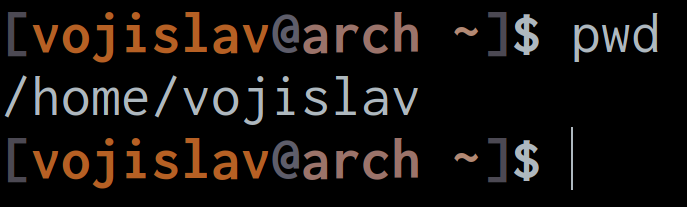
\includegraphics[scale=0.35]{pwd}
	\caption{Primer \texttt{pwd} komande}
\end{figure}
\begin{figure}[H]
	\centering
	
\includegraphics[scale=0.35]{cd}
	\caption{Primer \texttt{cd} komande}
\end{figure}
\begin{figure}[H]
	\centering
	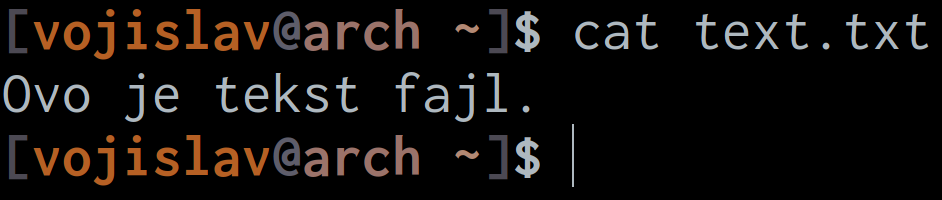
\includegraphics[scale=0.35]{cat}
	\caption{Primer \texttt{cat} komande}
\end{figure}